\documentclass[border=10pt]{standalone}
% \documentclass{article}
\usepackage{tikz}
\usetikzlibrary{arrows,decorations.pathmorphing,backgrounds,positioning,fit,petri}
\tikzstyle{particle} = [thick, fill=black!10]

\usepackage[T1]{fontenc}
\usepackage{dsfont}
\usepackage[utopia, greeklowercase=upright]{mathdesign}
\usepackage{amsmath}

\begin{document}

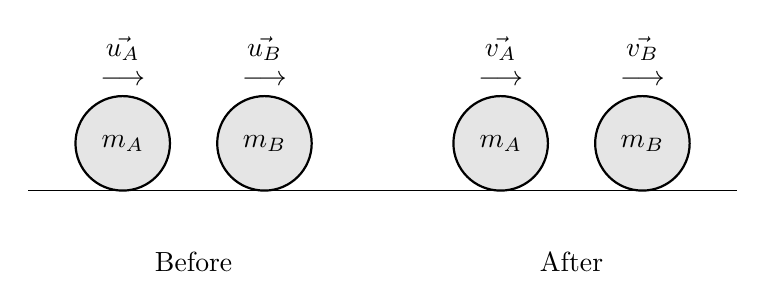
\begin{tikzpicture}[scale=1.2]

	\draw (0,0) -- (7.5,0);

	\draw[particle] (1,0.5) circle (0.5) node {$m_{A}$}
		++ (0,0.5) node[above] {$\longrightarrow$}
		++(0,0.5) node {$\vec{u_{A}}$};
	\draw[particle] (2.5,0.5) circle (0.5) node {$m_{B}$}
		++ (0,0.5) node[above] {$\longrightarrow$}
		++(0,0.5) node {$\vec{u_{B}}$};
	\draw[particle] (5,0.5) circle (0.5) node{$m_{A}$}
		++ (0,0.5) node[above] {$\longrightarrow$}
		++(0,0.5) node {$\vec{v_{A}}$};
	\draw[particle] (6.5,0.5) circle (0.5) node{$m_{B}$}
		++ (0,0.5) node[above] {$\longrightarrow$}
		++(0,0.5) node {$\vec{v_{B}}$};
	\node[align=center] at (1.75,-0.75) {Before};
	\node[align=center] at (5.75, -0.75) {After};

\end{tikzpicture}

\end{document}